\documentclass[pdftex,12pt,a4paper]{scrartcl}
\usepackage{graphicx}


\title{Software Architecture and Engineering}
\subtitle{Project Part 1: Social Network Modelling}
\date{March 28, 2015}
\author{Groupname: RMS -- Michael Alan Chang, Rik Melis, Simon T{\H o}dtli}

\begin{document}
\maketitle

{\bf A list of details from the project description that cannot be expressed in the UML model (Figure \ref{class_diagram})}
\begin{itemize}
  \item A friendship arrangement is always mutual.
  \item If you follow an actor and their content is visible to you (i.e. not blocked), then that content is presented on your newsfeed.
  \item If user A has blocked user B, then user B cannot see any of the content posted by user A.
  \item Specifically for messages, we add the recipient of the message to the privacy circles that the message is made available for.  For example, for 1-to-1 private message, the privacy circle would be `private', and the recipient of the message would be added to the private set.
  \item Privacy circle settings are implemented as is described in the assignment specifications.
  \item The ID signature encapsulates all the information required to identify the user, whether is a username, an email address, etc.
  \item Adminstrators of a group must also be a member of the group.
  \item On a user by user basis, the modifier of posted content is always the sender of a content. For a group, the modifiers of content are only administrators of the group.
  \item The process (dynamic) of adding people to a group can only be done by adminstrators.
  \item For the content of the group, the privacy settings are restricted to private and public. In other words, the content is either open to only the group members or to everyone un the social network universe.
\end{itemize}

\begin{figure}
\centering
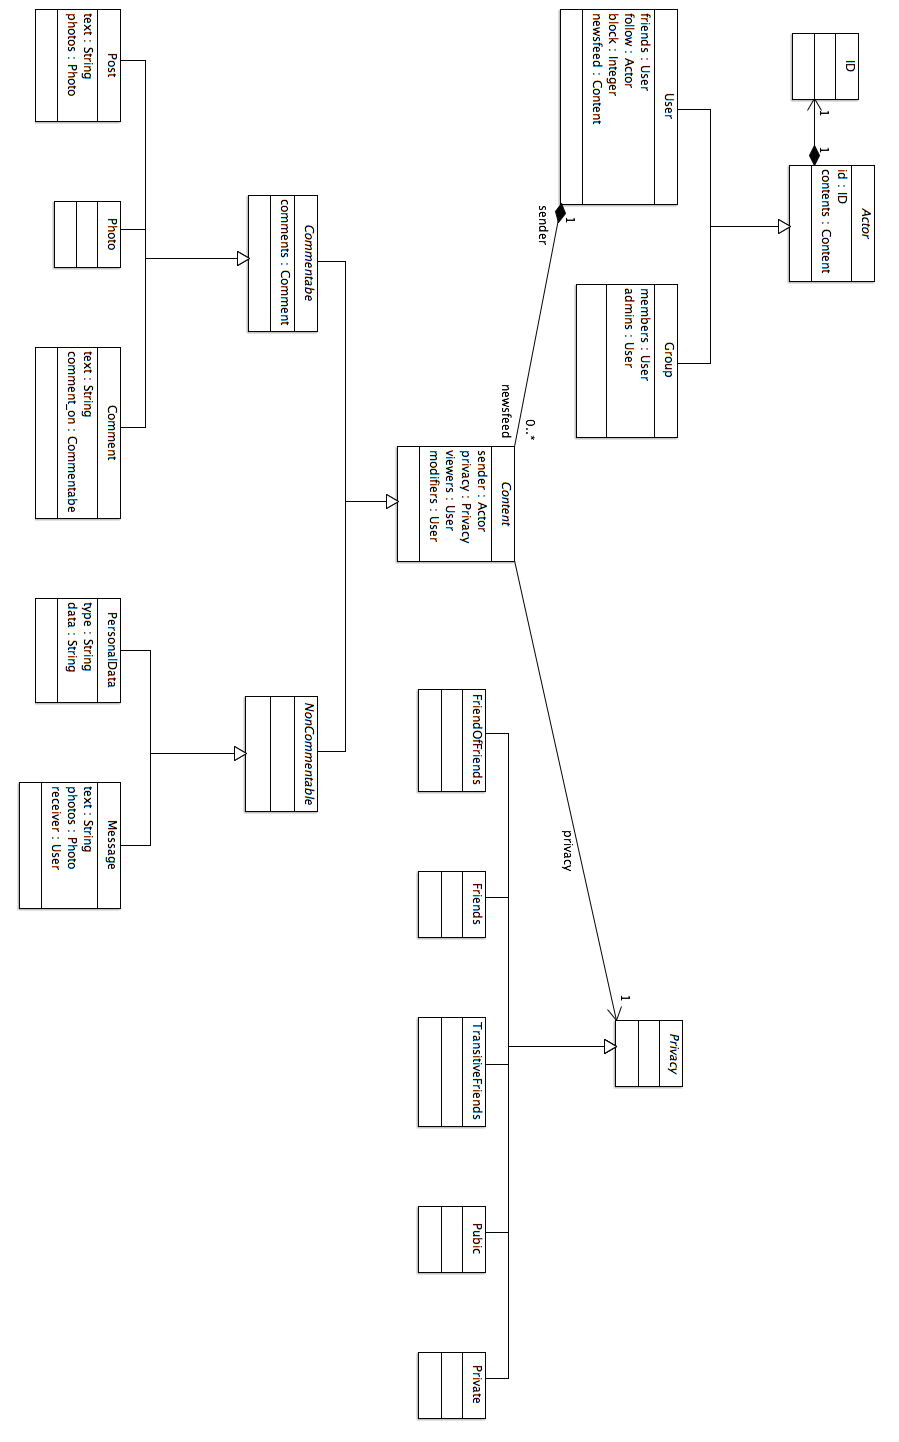
\includegraphics[scale=0.44]{classdiagram.png}
\caption{UML class diagram}
\label{class_diagram}
\end{figure}

\newpage
{\bf General Explanation of Design Decisions}
\begin{itemize}
  \item The type of the personal data cannot be repeated in a single profile. For example, a single user cannot have two birthdates or two home addresses.
  \item Groups and individual users utilize the same privacy circle classes. For individual users, the privacy settings are used exactly as they are described in the project specifications. For the groups, if some content is public, then all users of the social network can view the content (unless they are blocked) . On the other hand, all of the other four privacy settings -- friends, friends of friends, transitive friends, and private -- are interpreted as private to the members of the group.
  \item We addressed privacy settings as generally as possible. In Part D4, it is stated that `If a post or message includes photos, the photos are visible at least to all the people that can view the post'. Our privacy rules strictly follow this statement, and we further extend this statement to comments. This is described by the following statement: `If a commentable content is commented on, the comments are visible at least to all the people that can view the content that is being commented on.' We didn't make further restrictions on the privacy settings of recursive content (i.e. comments, and photos in posts and messages) because this is not declared in the project description.
  \item	If user A is blocked by user B, user A cannot receive even a private message from User B. This is reinforced by the assertion made in D7: `A user cannot see any content created by a user that blocks them.'
\end{itemize}

{\bf Alloy model}
\begin{itemize}
  \item Figure \ref{alloy_model} displays a general instance of our alloy model. For generating this instance we runned the empty predicate {\it show}:\\
\texttt{run show for exactly 4 ID, exactly 2 Group, exactly 2 User, exactly 1 Message, exactly 1 PersonalData, exactly 1 Comment, exactly 1 Photo, exactly 1 Post, exactly 2 MyString}
\end{itemize}

\begin{figure}
\centering
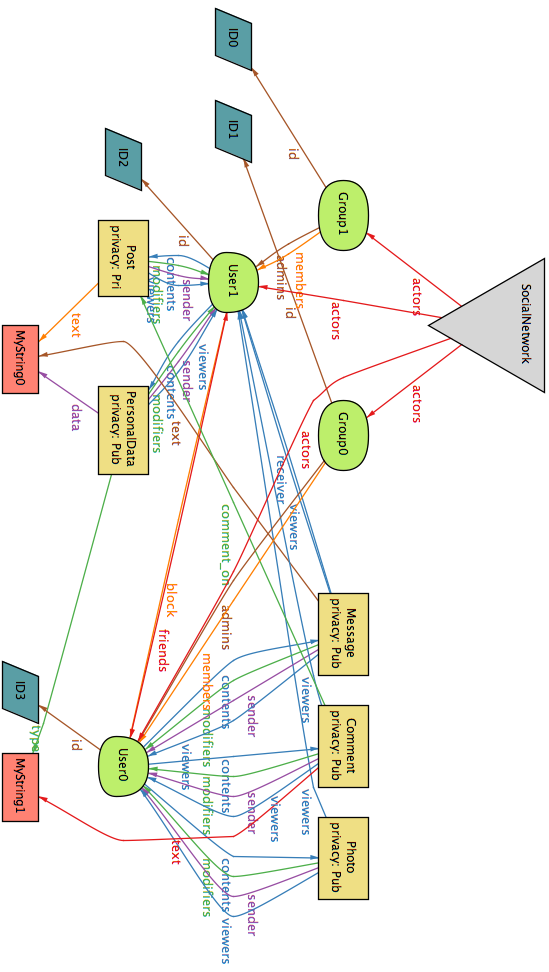
\includegraphics[scale=0.65]{alloy_model.png}
\caption{Alloy model}
\label{alloy_model}
\end{figure}

\newpage
{\bf A list of properties from Task D that you were not able to check, each with a short explanation why the property does not hold }
\begin{itemize}
  \item There were no properties that we were not able to verify.
\end{itemize}

{\bf A list of instances from Task E that you were not able to produce, each with a short explanation why the instance is not feasible } 

\begin{itemize}
  \item Part E6 is not feasible as it is in direct contradiction from the assertion made in D4. To reiterate, D4 states that photos in a post or message are visible at least to all the people that can view the post. E6 asks us the find a user that can see the post, but not the photo in the post. In this regard, it is impossible to have a scenario where someone can view a post but not the photo in the post as is described in E6.
\end{itemize}

{\bf Diagrams of all the generated instances from Task E}\\

To make the diagrams clear, we left all the instances and relations that are irrelevant for the instance. To see to entire diagram, you can run the predicates in the alloy file. The run statements are given in comments.

\begin{enumerate}
  \item A comment chain that is 5 comments long\\
  \begin{center}
  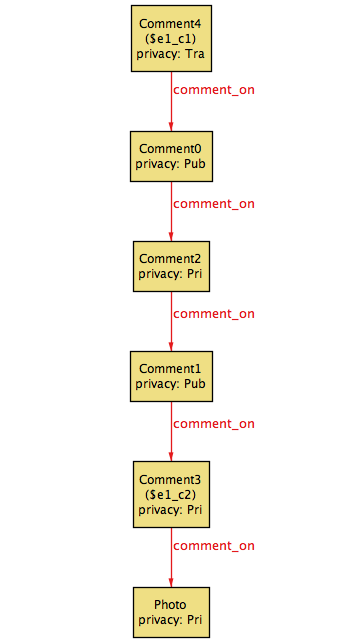
\includegraphics[scale=0.5]{e1.png}
  \end{center}
  \item 3 users that form 7 different groups, each with a different set of members
  \begin{center}
  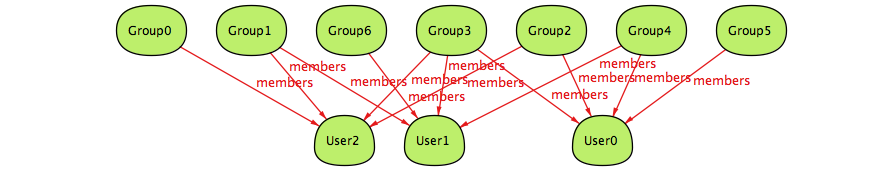
\includegraphics[scale=0.5]{e2.png}
  \end{center}
  \item 4 users, where each has at least one friend, but not everyone is a transitive friend of everyone else
  \begin{center}
  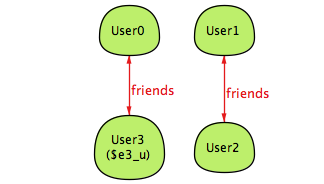
\includegraphics[scale=0.5]{e3.png}
  \end{center}
  \item A user that can see a post of a user that is a friend of friend (but not a direct friend), which has privacy level `friend of friend' and includes a photo from a fourth user
  \begin{center}
  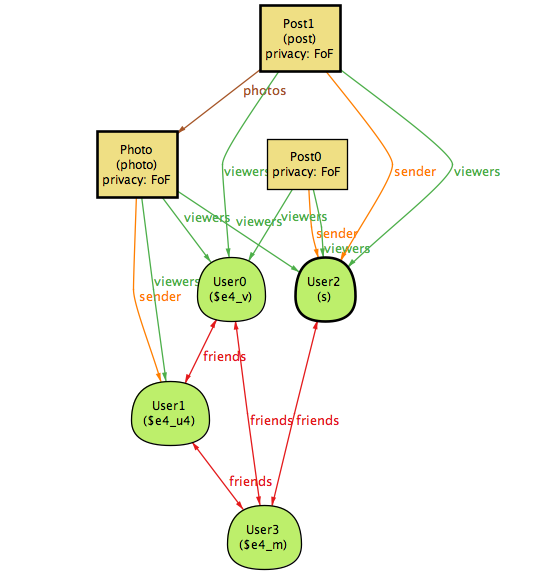
\includegraphics[scale=0.5]{e4.png}
  \end{center}
  \item A post that includes a photo created not by the poster, where the photo is not public
  \begin{center}
  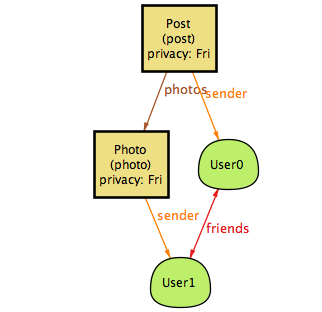
\includegraphics[scale=0.6]{e5.png}
  \end{center}
  \item A post with the privacy level `friends of friends', which includes a photo created by a friend of the creator of the post. Some friend of the creator of the post must be able to see the post, but not the photo\\
  {\bf infeasible}

\end{enumerate}

\end{document}

